\section{Transporting the evolution of the entropic rule}
\label{sec:entropic-evolution}
Advancing a state and advancing its changing transport rule impose different
closure requirements. For an exact finite transfer $d_{k+1}=A_kd_k$, the
change $a_k=d_{k+1}-d_k$ satisfies
\begin{equation}
 a_{k+1}=A_{k+1}a_k+(A_{k+1}-A_k)d_k.
 \label{eq:evolution-cocycle}
\end{equation}
Freezing $A_k$ removes the second contribution. Representing that contribution
does not by itself make its execution cheaper. We examine these two issues
in positive-kernel Sinkhorn iteration, where the evolving geometry admits
an explicit nonlinear closure and, for a structured family, an exact
projective linear lift.

Sinkhorn scaling and its interpretation as entropic optimal transport are
established \cite{peyre}. Its local spectrum and accelerated variants have
also been studied extensively \cite{lehmann}. The results below organize
its conditional geometry around the present state-and-rule closure question;
we do not claim priority for matrix scaling, exponential reweighting,
projective matrix powers, or nonlinear reduced modeling.

\subsection{An instantaneous metric determined by the displacement}
Let $K\in\R_{>0}^{m\times n}$ and let $a,b$ be positive marginals of equal
total mass. All exponentials, logarithms, and vector quotients below are
componentwise. In log column-scaling coordinates, one full pass is
\begin{equation}
 x(y)=\log a-\log(Ke^y),\qquad
 F(y)=\log b-\log(K^Te^{x(y)}).
 \label{eq:entropic-map}
\end{equation}
The next row scaling is determined by $y$ and carries no independent memory
in this ordinary algorithm. This elimination is specific to its phase
contract; it does not justify deleting independent splitting memories.
The map has the gauge symmetry $F(y+\gamma\mathbf1)=F(y)+\gamma\mathbf1$.

Set $u=e^{x(y)}$, $v=e^y$, and define
\begin{equation}
 \Pi=\diag(u)K\diag(v),\quad c=\Pi^T\mathbf1,\quad
 P=\diag(a)^{-1}\Pi,\quad Q=\diag(c)^{-1}\Pi^T.
 \label{eq:entropic-conditionals}
\end{equation}
Thus $\Pi\mathbf1=a$, while $c$ is the current column marginal. Both
$P$ and $Q$ are row stochastic.

\begin{proposition}[Moving conditional metric]
\label{prop:entropic-metric}
At every finite state,
\begin{equation}
 J(y)=DF(y)=QP,\qquad
 \diag(c)J=\Pi^T\diag(a)^{-1}\Pi.
 \label{eq:entropic-metric}
\end{equation}
Consequently $J$ is self-adjoint and positive semidefinite in the
$c$-weighted inner product, with spectrum in $[0,1]$. For the actual
displacement $d=F(y)-y$,
\begin{equation}
 c=b\odot e^{-d}. \label{eq:entropic-metric-displacement}
\end{equation}
\end{proposition}
\begin{proof}
Differentiation gives $Dx[h]=-Ph$ and $DF[h]=QPh$.
The second identity in \eqref{eq:entropic-metric} follows by multiplication.
Conjugating $J$ by $\diag(\sqrt c)$ gives $B^TB$, where
$B=\diag(a)^{-1/2}\Pi\diag(c)^{-1/2}$. Jensen's inequality and the two
marginal identities imply
$\norm{Ph}_a\leq\norm h_c$ and $\norm{Qk}_c\leq\norm k_a$.
The spectrum therefore lies in $[0,1]$. Finally,
$c=v\odot(K^Tu)$ and $e^{F(y)}=b/(K^Tu)$ imply
\eqref{eq:entropic-metric-displacement}.
\end{proof}

The displacement determines the metric, but not the full conditional
coupling. Moreover, an instantaneous symmetric chart is not a fixed chart:
writing $W_k=\diag(\sqrt{c_k})$ introduces $W_{k+1}J_kW_k^{-1}$ when a
tangent is carried between successive whitened coordinates. Positive
instantaneous spectra do not imply that successive propagators commute.

This also distinguishes the entropic mechanism from a possible Meyer
phase mode. On an interior disk branch, a single whitened longitudinal
primal/memory block has the form
\[
 \frac{1}{1+\sigma^2}
 \begin{pmatrix}1&-\sigma\\\sigma&1\end{pmatrix},
 \qquad \lambda_\pm=\frac{1\pm i\sigma}{1+\sigma^2}.
\]
That branch calculation is not a diagonalization of the full coupled map,
but it shows why its retained phase evolution should not be inferred from
Sinkhorn's conditional averaging structure. The complete-state principle
transfers; the primitive mechanism must be derived for the new map.

\subsection{Exact finite evolution of the state and rule}
\begin{theorem}[Closed conditional evolution]
\label{thm:entropic-evolution}
For any displacement $h$, define
\begin{equation}
 e=-\log(Pe^h),\qquad g=-\log(Qe^e).
 \label{eq:entropic-increment}
\end{equation}
Then $x(y+h)-x(y)=e$, $F(y+h)-F(y)=g$, and the new conditional geometry is
\begin{align}
 P^+&=\diag(Pe^h)^{-1}P\diag(e^h),\nonumber\\
 Q^+&=\diag(Qe^e)^{-1}Q\diag(e^e).
 \label{eq:entropic-rule-update}
\end{align}
If $h=d=F(y)-y$, the recurrence
$(y,d,P,Q)^+=(y+d,g,P^+,Q^+)$ reproduces ordinary Sinkhorn evolution.
Equivalently,
\begin{equation}
 \Pi^+=\diag(e^e)\Pi\diag(e^d),\qquad
 c^+=b\odot e^{-g}.
 \label{eq:entropic-coupling-update}
\end{equation}
\end{theorem}
\begin{proof}
Substitute $e^{y+h}=v\odot e^h$ into the first normalization in
\eqref{eq:entropic-map}. Division by its old normalizer gives $e$.
The same substitution $e^{x+e}=u\odot e^e$ in the second normalization
gives $g$. Dividing the reweighted rows of each conditional by their row
sums yields \eqref{eq:entropic-rule-update}; multiplication of the two
diagonal factors gives \eqref{eq:entropic-coupling-update}. The actual
displacement obeys $g=F(y+d)-F(y)=F(y+d)-(y+d)$, proving the recurrence.
\end{proof}

Initialization must be consistent with the given $K,a,b$; arbitrary
independent stochastic $P,Q$ need not describe that problem. The update
preserves every cross ratio
$\Pi_{ij}\Pi_{\ell k}/(\Pi_{ik}\Pi_{\ell j})$, which equals the
corresponding ratio of $K$. The moving geometry remains in a fixed diagonal
scaling orbit. Storing its full conditionals is redundant and costs
$O(mn)$ per update, the same order as a dense ordinary pass. Keeping only
their diagonal factors saves storage but still requires the kernel actions
for normalization. Exact closure has not yet supplied economical composition.

For a row-stochastic $R$, let
\[
 \overline R(h)=\int_0^1
   \diag(Re^{th})^{-1}R\diag(e^{th})\,dt.
\]
The fundamental theorem of calculus gives
$\log(Re^h)=\overline R(h)h$. Thus the exact finite transfer is
$g=A(y,h)h$ with $A(y,h)=\overline Q(e)\overline P(h)$, a product of
stochastic matrices. Along the actual trajectory it satisfies
\eqref{eq:evolution-cocycle}. The integrals define a proof representation;
\eqref{eq:entropic-increment} evaluates the increment without quadrature.
This secant representation is exact on the specified displacement and
is not asserted to be unique.

\subsection{The nonlinear sources and their finite-horizon bounds}
Define the log-moment remainder
\[
 L_R(h)=\log(Re^h)-Rh,\qquad
 \operatorname{osc}(h)=\max_j h_j-\min_j h_j.
\]
Substitution in \eqref{eq:entropic-increment} yields the exact identity
\begin{equation}
 F(y+h)-F(y)-J(y)h=Q L_P(h)-L_Q(e).
 \label{eq:entropic-sources}
\end{equation}
The changing primitive sources are explicit, as in the coupled disk
construction, although their algebra and transport costs differ.

\begin{theorem}[First- and second-order entropic remainder bounds]
\label{thm:entropic-remainders}
For every finite $y,h$, put $R=\operatorname{osc}(h)$. Then
\begin{align}
 \norm{F(y+h)-F(y)-J(y)h}_\infty&\leq R^2/8,
 \label{eq:entropic-linear-bound}\\
 \norm{F(y+h)-F(y)-J(y)h-\tfrac12D^2F(y)[h,h]}_\infty
 &\leq 11R^3/96.
 \label{eq:entropic-quadratic-bound}
\end{align}
The second derivative has the finite conditional-moment expression
\begin{equation}
 D^2F[h,k]=QP(h\odot k)-2Q\{(Ph)\odot(Pk)\}
                    +(QPh)\odot(QPk).
 \label{eq:entropic-hessian}
\end{equation}
\end{theorem}
\begin{proof}
For any probability row $(\omega_j)$, the second derivative of
$\ell(t)=\log\sum_j\omega_je^{th_j}$ is the variance of $h$ under the
tilted row probabilities. It lies in $[0,R^2/4]$, so
$0\leq L_R(h)_i\leq R^2/8$. The components of $e$ in
\eqref{eq:entropic-increment} lie between $-\max h$ and $-\min h$.
Both nonnegative terms in \eqref{eq:entropic-sources} therefore lie in
$[0,R^2/8]$, proving \eqref{eq:entropic-linear-bound}.

For the cubic remainder, differentiate the first half-step along $y+th$.
Each $x_i'$ lies in an interval of length $R$, each $x_i''$ in
$[-R^2/4,0]$, and $|x_i'''|\leq R^3/4$. The last estimate follows from
$|\mathbb E(X-\mathbb EX)^3|\leq R\operatorname{Var}(X)$.
The third derivative of the second log-sum-exp is, up to sign, the sum
of an expected $x'''$, three times $\operatorname{Cov}(x',x'')$, and the
third central moment of $x'$. Their absolute values are bounded by
$R^3/4$, $3R^3/16$, and $R^3/4$, respectively. Taylor's integral remainder
is at most $(11R^3/16)/6$. Differentiating twice and collecting the two
conditional covariance terms gives \eqref{eq:entropic-hessian}.
\end{proof}

These are global displacement bounds for a finite positive kernel, not
asymptotic notation. They need not be sharp. They also identify a limited
polynomial obstruction: if a row has positive weights and $h$ is nonconstant
on its support, $\ell(t)$ cannot agree with a finite-degree polynomial on
any open interval. It is real analytic on the real line and grows at most
linearly at either infinity. Such agreement would force an affine function,
contradicting $\ell''(0)>0$. This argument concerns that primitive in that
coordinate. It does not rule out cancellations in the full pass, finite
polynomial approximation, nonlinear decoding, or another finite lift.

Use the quotient norm $\norm h_q=\operatorname{osc}(h)/2$. Stochasticity
of $DF$ implies that $F$ is globally nonexpansive in this norm. Let $s_0=0$
and let a retained model give $s_{j+1}$, while $T_y(s_j)$ is the complete
first- or second-order Taylor displacement of $F(y+s_j)-y$. If
$\delta_j=\norm{T_y(s_j)-s_{j+1}}_q$, telescoping gives
\begin{equation}
 \norm{F^H(y)-(y+s_H)}_q
 \leq\sum_{j=0}^{H-1}\{\delta_j+\mathcal R(s_j)\},
 \quad
 \mathcal R(s)=
 \begin{cases}
  \operatorname{osc}(s)^2/8,&\text{linear},\\
  11\operatorname{osc}(s)^3/96,&\text{quadratic}.
 \end{cases}
 \label{eq:entropic-path-bound}
\end{equation}
The term $\delta_j$ includes escape from the retained state space. The
bound assumes exact arithmetic; it is not a certified floating-point
objective-gap estimate.

\subsection{Exact projective closure with a changing derivative}
The fractional-linear examples in Section~\ref{sec:general-geometry}
were constructed from compatible scalar dynamics. Here the same type of
lift follows from an established nonlinear algorithm without fitting a
componentwise rational surrogate.

\begin{proposition}[Two-by-two Sinkhorn lift]
\label{prop:sinkhorn-projective}
For $K=\left(\begin{smallmatrix}p&q\\r&s\end{smallmatrix}\right)>0$,
the quotient $t=v_1/v_2$ obeys $t^+=(At+B)/(Ct+D)$, where
\begin{align*}
 A&=(b_1/b_2)(q a_1r+s a_2p),&
 B&=(b_1/b_2)qs(a_1+a_2),\\
 C&=pr(a_1+a_2),&D&=p a_1s+r a_2q.
\end{align*}
With $M=\left(\begin{smallmatrix}A&B\\C&D\end{smallmatrix}\right)$,
\begin{equation}
 t_H=\frac{(M^H)_{11}t_0+(M^H)_{12}}
              {(M^H)_{21}t_0+(M^H)_{22}},\qquad
 \frac{dt_H}{dt_0}=
 \frac{\det(M)^H}{\{(M^H)_{21}t_0+(M^H)_{22}\}^2}.
 \label{eq:sinkhorn-projective-power}
\end{equation}
If $ps\ne qr$, the one-pass derivative
$\det(M)/(Ct+D)^2$ is nonconstant in $t$.
\end{proposition}
\begin{proof}
In any scale gauge, insert
$u_1=a_1/(pt+q)$ and $u_2=a_2/(rt+s)$ into
$t^+=(b_1/b_2)(qu_1+su_2)/(pu_1+ru_2)$ and clear denominators.
Composition of fractional-linear maps multiplies their homogeneous
matrices. Differentiating the resulting fraction proves the second formula;
$\det(M)=(b_1/b_2)a_1a_2(ps-qr)^2$.
\end{proof}

Cayley--Hamilton expresses $M^H=\alpha_HM+\beta_HI$, and normalized binary
powering needs $O(\log H)$ fixed-size matrix products. This transports a
changing physical derivative using a constant lifted operator. Exact
rational bit lengths and floating-point conditioning still require attention.
The lift describes quotient states. To recover the ordinary post-column
coupling after $H$ passes, advance through $H-1$ and perform the final
row/column pair in a consistent gauge; the row-normalized output phase used
below is obtained by evaluating the next row normalization.

The closure extends to arbitrary dimensions with supplied exact structure
\begin{equation}
 K_{ij}=r_i C_{g(i),h(j)}s_j.
 \label{eq:sinkhorn-block-kernel}
\end{equation}
Let $A_g=\sum_{i:g(i)=g}a_i$, $B_h=\sum_{j:h(j)=h}b_j$.
After one full pass, $v_j=(b_j/s_j)w_{h(j)}/B_{h(j)}$, and substitution
gives the invariant reduced map
\begin{equation}
 w^+=B\big/\{C^T(A/(Cw))\}.
 \label{eq:sinkhorn-block-map}
\end{equation}
For arbitrary initial $v$, use $w_h=\sum_{j:h(j)=h}s_jv_j$ for the entry
pass. Two groups on each side reduce exactly to
Proposition~\ref{prop:sinkhorn-projective}. Within-manifold derivative
evolution follows the same lift; arbitrary initial perturbations also
require the derivative of the entry map. Discovery or verification of the
block structure must be charged, and rank two alone does not imply
\eqref{eq:sinkhorn-block-kernel}.

\subsection{A bounded changing-rule model for general kernels}
We acquire a weighted Krylov basis $U$ from the actual displacement, with
$U^T\diag(c/\sum c)U=I$ and $c^TU=0$. Conditional kernel products give
the complete vectors $JU$ and $D^2F[U_i,U_j]$; their weighted projections
define a reduced quadratic map
\begin{equation}
 z^+=\rho+Hz+\tfrac12G[z,z],\qquad
 D\widehat F(z)=H+G[z,\cdot].
 \label{eq:sinkhorn-reduced-rule}
\end{equation}
Its derivative evolves during the rollout. This is a nonlinear polynomial
state model, not a polynomial of one frozen physical Jacobian. Its primitive
construction and the exact lifted polynomial in
\eqref{eq:sinkhorn-projective-power} are distinct realizations of closure.

Every modeled step evaluates the complete-vector polynomial and its
projection defect for \eqref{eq:entropic-path-bound}, with no further kernel
action. We compare the linear four-direction control, the matched quadratic
four-direction model, and a cheaper quadratic two-direction version.
The maximum horizon is 128; the accumulated bound must be at most $0.05$
times the predicted quotient displacement. Minimum accepted horizons are
16 for the linear and two-direction models, and 32 for quadratic four.
Eight ordinary passes precede acquisition and follow an unsuccessful
acquisition. An accepted advance triggers a fresh acquisition.

A proposal is additionally evaluated with the original kernel and accepted
only when the actual maximum relative marginal error decreases. Otherwise
the cached ordinary step is taken. These checks, unsuccessful acquisitions,
all tensors and bounds, rejected work, and reconstruction are timed.
No fixed-point solve or future trajectory is used. The implementation uses
normalized scaling arithmetic for finite positive kernels; it is not a
fully stabilized log-domain solver for arbitrary underflow or sparse support.

\subsection{Measured application and its cost limit}
We use six positive-kernel families at $n=256,1024,2048$: a positive
lognormal matrix, two line Gaussian kernels, and three plane Gaussian
kernels. Line marginals shift with the seed; plane supports and masses
are sampled independently. Settings were screened on seed zero and held
fixed for seeds one and two. Five repetitions per method and problem
are shuffled after warm-up on the M4 CPU with single-thread BLAS.
The output phase normalizes rows exactly and stops at
$\max_j|c_j/b_j-1|\leq10^{-9}$. Common input-kernel construction is
excluded; all method-specific setup, unsuccessful work, checks, and
scaling-factor reconstruction are included. Dense plan materialization
is excluded for every method.
All 720 general solves and 120 structured solves reach the target.
This is matched marginal accuracy, not a certified objective-gap comparison.

\begin{table}[!hbp]\centering\small
\begin{tabular}{lrrrr}\toprule
Problem & Ordinary & Frozen 4 & Changing 4 & Changing 2\\\midrule
Line, $\varepsilon=0.02$ & 85.66 & 62.29 & 80.11 & 80.22\\
Line, $\varepsilon=0.003$ & 547.80 & 349.35 & 493.13 & 426.58\\
Plane, $\varepsilon=0.03$ & 57.37 & 49.11 & 58.56 & 61.41\\
Plane, $\varepsilon=0.006$ & 281.61 & 191.12 & 276.25 & 243.55\\
Plane, $\varepsilon=0.003$ & 564.03 & 380.82 & 536.28 & 459.07\\
\bottomrule\end{tabular}
\caption{Complete solve times in milliseconds at $n=2048$, reported as
the median of per-seed five-repeat medians. The matched four-direction
comparison isolates the added changing-rule model; the two-direction
version also changes representation capacity.}\label{tab:entropic-cost}
\end{table}


The two-direction changing-rule model is $1.13$--$1.33\times$ faster
than ordinary iteration on the three narrow-kernel cases at $n=1024$,
and $1.16$--$1.28\times$ at $n=2048$. It loses on every nontrivial
$n=256$ case. At $n=2048$ the frozen control is faster than either
changing-rule variant on all five nontrivial cases. The positive
lognormal control finishes before acquisition begins; its timing
differences are noise. These controls do not establish superiority over
Anderson, overrelaxed Sinkhorn, continuation, or specialized OT solvers.

\begin{figure}[tb]\centering
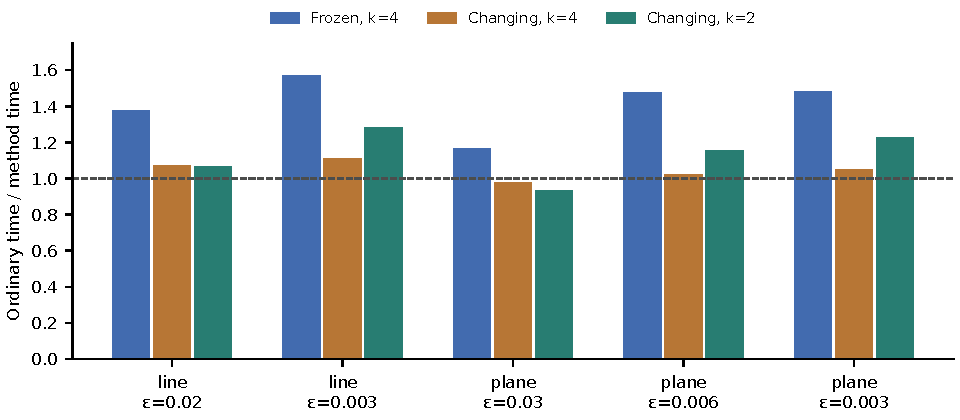
\includegraphics[width=\linewidth]{figures/entropic_cost.pdf}
\caption{General-kernel speedups at $n=2048$. Values above one are faster
than ordinary iteration. Ratios are summarized within seed before
aggregation. Better modeling of the evolving rule does not yet offset
its acquisition cost relative to the frozen control.}\label{fig:entropic-cost}
\end{figure}

For the narrow-line case, median actual map evaluations are 198,186,193
for frozen four, changing four, and changing two, respectively. Their
kernel-vector products are 648,1114,686. Batched products need not have
the same per-vector cost, but these counts explain why fewer full passes
are insufficient evidence of a faster method.

An independent diagnostic holds the four-direction basis fixed and
compares horizons 16 and 32 at ordinary prefixes 8,32,128, for size 128
and seeds zero and one. Already-converged anchors are skipped.
Of 52 paired comparisons, the quadratic model improves state prediction
in 39 and the projected endpoint-derivative prediction in 36. Fifty
pairs complete for both models; two unrestricted quadratic rollouts do
not complete. No evaluated finite-trajectory bound is violated. True
future states are used only for this untimed diagnostic, never by the solver.

\begin{figure}[tb]\centering
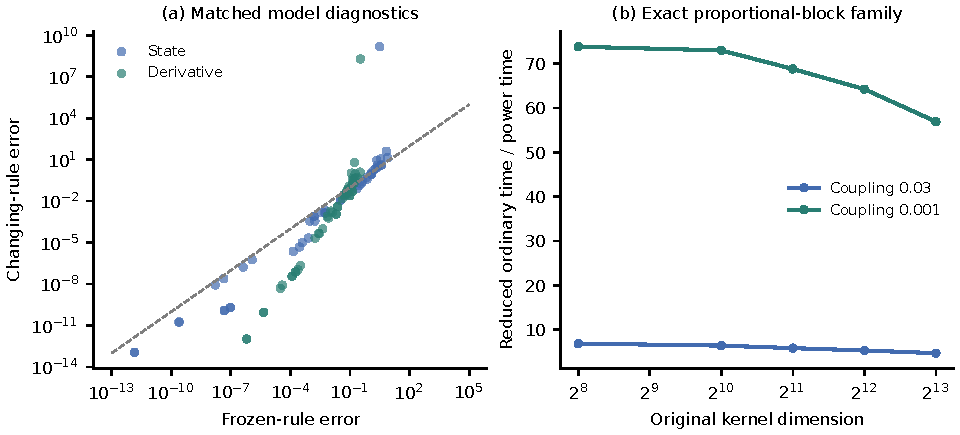
\includegraphics[width=\linewidth]{figures/entropic_closure.pdf}
\caption{(a) All 50 completed pairs in the unrestricted matched-model
diagnostic; below the diagonal favors the changing rule. Two additional
quadratic rollouts fail to complete. Derivative errors concern the same
anchor-projected operator, not a full operator-norm certificate.
(b) Exact projective-power speedups over ordinary iteration using the
same supplied block reduction, including full scaling-factor readout.}
\label{fig:entropic-closure}\end{figure}

For the exact two-group family, both comparators use
\eqref{eq:sinkhorn-block-map}. The power method increases its finite
horizon geometrically and checks the actual reduced marginal residual.
Across original dimensions 256 through 8192, the speedup is
$4.7$--$6.9\times$ for block coupling $.03$ and
$56.9$--$73.8\times$ for coupling $.001$. The latter reduced ordinary
runs take approximately 14--15 ms, versus $.19$--$.26$ ms for powers
and reconstruction. This family validates economical exact closure;
it does not demonstrate discovery of that structure on arbitrary kernels.

A separate earlier transfer study, retained with the source, compared
fixed polynomial, discovery, and Anderson methods on 24 image-mass and
Gaussian-mixture problems. It used a different marginal norm, checking
cadence, sizes, and acquisition policy. Its timings are not pooled here.
Anderson was generally stronger there; the present experiment isolates
the cost of carrying the evolving rule rather than establishing a new
best general Sinkhorn solver.


\subsection{What the application establishes}
The exact conditional recurrence establishes transportability of the rule's
evolution. The projective family establishes inexpensive composition under
a specific invariant representation. The general quadratic model establishes
useful prediction of changing geometry and some acceleration over ordinary
execution, but the frozen control remains cheaper in the retained large
general-kernel comparisons. This separates a representation theorem, a
prediction result, and a computational advantage. None implies the other
two without its own argument.

The Sinkhorn input kernel, marginals, state contract, and conditional
derivatives are supplied mathematical structure. Acquiring their reduced
responses is not discovery of those ingredients from an arbitrary black box.
Likewise, a fixed lifted matrix can encode changing physical geometry,
whereas repeatedly rebuilding an accurate local rule can cost more than
the ordinary work it replaces. Economical closure of the moving relationships,
including acquisition and readout, is the research target.
